% flashcards-title: Six quarter groups in one and one half
% flashcards-desc: A bar of length one and one half is divided into six equal quarter-length segments, grouped by alternating fill and hatch.
\documentclass[dvisvgm,tikz,border=8pt]{standalone}
\usetikzlibrary{arrows.meta,patterns}

\definecolor{qraNavy}{HTML}{17324D}
\definecolor{qraBlue}{HTML}{2B6CB0}
\definecolor{qraGold}{HTML}{B7791F}
\definecolor{qraPale}{HTML}{EAF2F8}
\definecolor{qraGray}{HTML}{5C6773}

\tikzset{
  qra axis/.style={draw=qraNavy, line width=1.2pt},
  qra tick/.style={draw=qraNavy, line width=1pt},
  qra guide/.style={draw=qraGray, densely dashed, line width=0.8pt},
  qra counter/.style={circle, draw=qraNavy, fill=qraPale, line width=0.9pt, minimum size=7mm, inner sep=0pt},
  qra label/.style={font=\sffamily\bfseries, text=qraNavy},
  qra small label/.style={font=\sffamily, text=qraNavy},
}

\begin{document}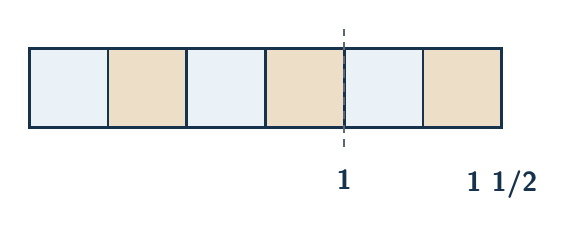
\begin{tikzpicture}[x=1cm,y=1cm]
\foreach \x in {0,2,4}{\fill[qraPale](\x,0)rectangle(\x+1,1);}
\foreach \x in {1,3,5}{\fill[qraGold!25](\x,0)rectangle(\x+1,1);}
\draw[qra axis](0,0)rectangle(6,1);\foreach \x in {1,...,5}{\draw[qra tick](\x,0)--(\x,1);}
\draw[qra guide](4,-.25)--(4,1.25);\node[qra label,below=5pt]at(4,-.25){1};\node[qra label,below=5pt]at(6,-.25){1 1/2};
\end{tikzpicture}\end{document}
